\documentclass{beamer}
\usepackage{listings}
\lstset{
    language=Python,
    basicstyle=\tiny\ttfamily,
    frame=single,
    commentstyle=\color{red},
}

% Theme and color settings
\usetheme{CambridgeUS}
\usecolortheme{default}

% Package imports
\usepackage{graphicx}
\usepackage{booktabs}
\usepackage{url}

% Title information
\title{Naïve Semantic Text Similarity Model}
\author{Zachary Parent}
\institute{UPC}
\date{\today}

\begin{document}

% Title frame
\begin{frame}
    \titlepage
\end{frame}

% Table of contents
\begin{frame}{Outline}
    \tableofcontents
\end{frame}

% Introduction
\section{Introduction}
\begin{frame}{Introduction}
    \begin{itemize}
        \item Semantic Text Similarity (STS) is crucial for many NLP tasks
        \item Challenge: Which features best capture semantic similarity?
        \item Our approach: Unbiased feature analysis using process pipeline permutations and Random Forests for feature analysis
    \end{itemize}
\end{frame}

% Approach
\section{Methodology}
\begin{frame}{Methodology}
    \begin{itemize}
        \item Approach
        \item Feature extraction
        \item Feature selection
        \item Model training
        \item Model evaluation
    \end{itemize}
\end{frame}

\subsection{Approach}
\begin{frame}{Approach}
    \begin{itemize}
        \item Naïve approach which requires no knowledge of the corpus
        \item Use categorized steps to process sentences in every permutation
        \begin{itemize}
            \item 520 permutations
            \item e.g. sentence\_to\_doc $\rightarrow$ \texttt{chunk\_NEs} $\rightarrow$ \texttt{remove\_stopwords} $\rightarrow$ \texttt{lemmatize\_tokens} $\rightarrow$ \texttt{get\_characters} $\rightarrow$ \texttt{get\_2grams}
        \end{itemize}
        \item Apply 4 similarity metrics to each permutation
        \begin{itemize}
            \item Jaccard, Cosine, Euclidean, Manhattan
        \end{itemize}
        \item Used Random Forest's feature importance capabilities
        \item Let the data guide feature selection
    \end{itemize}

\end{frame}

\subsection{Feature Extraction}
\begin{frame}{Feature Extraction}
    \begin{center}
        \Large Feature Extraction
    \end{center}
\end{frame}

\begin{frame}{Feature Extraction}
    \begin{center}
        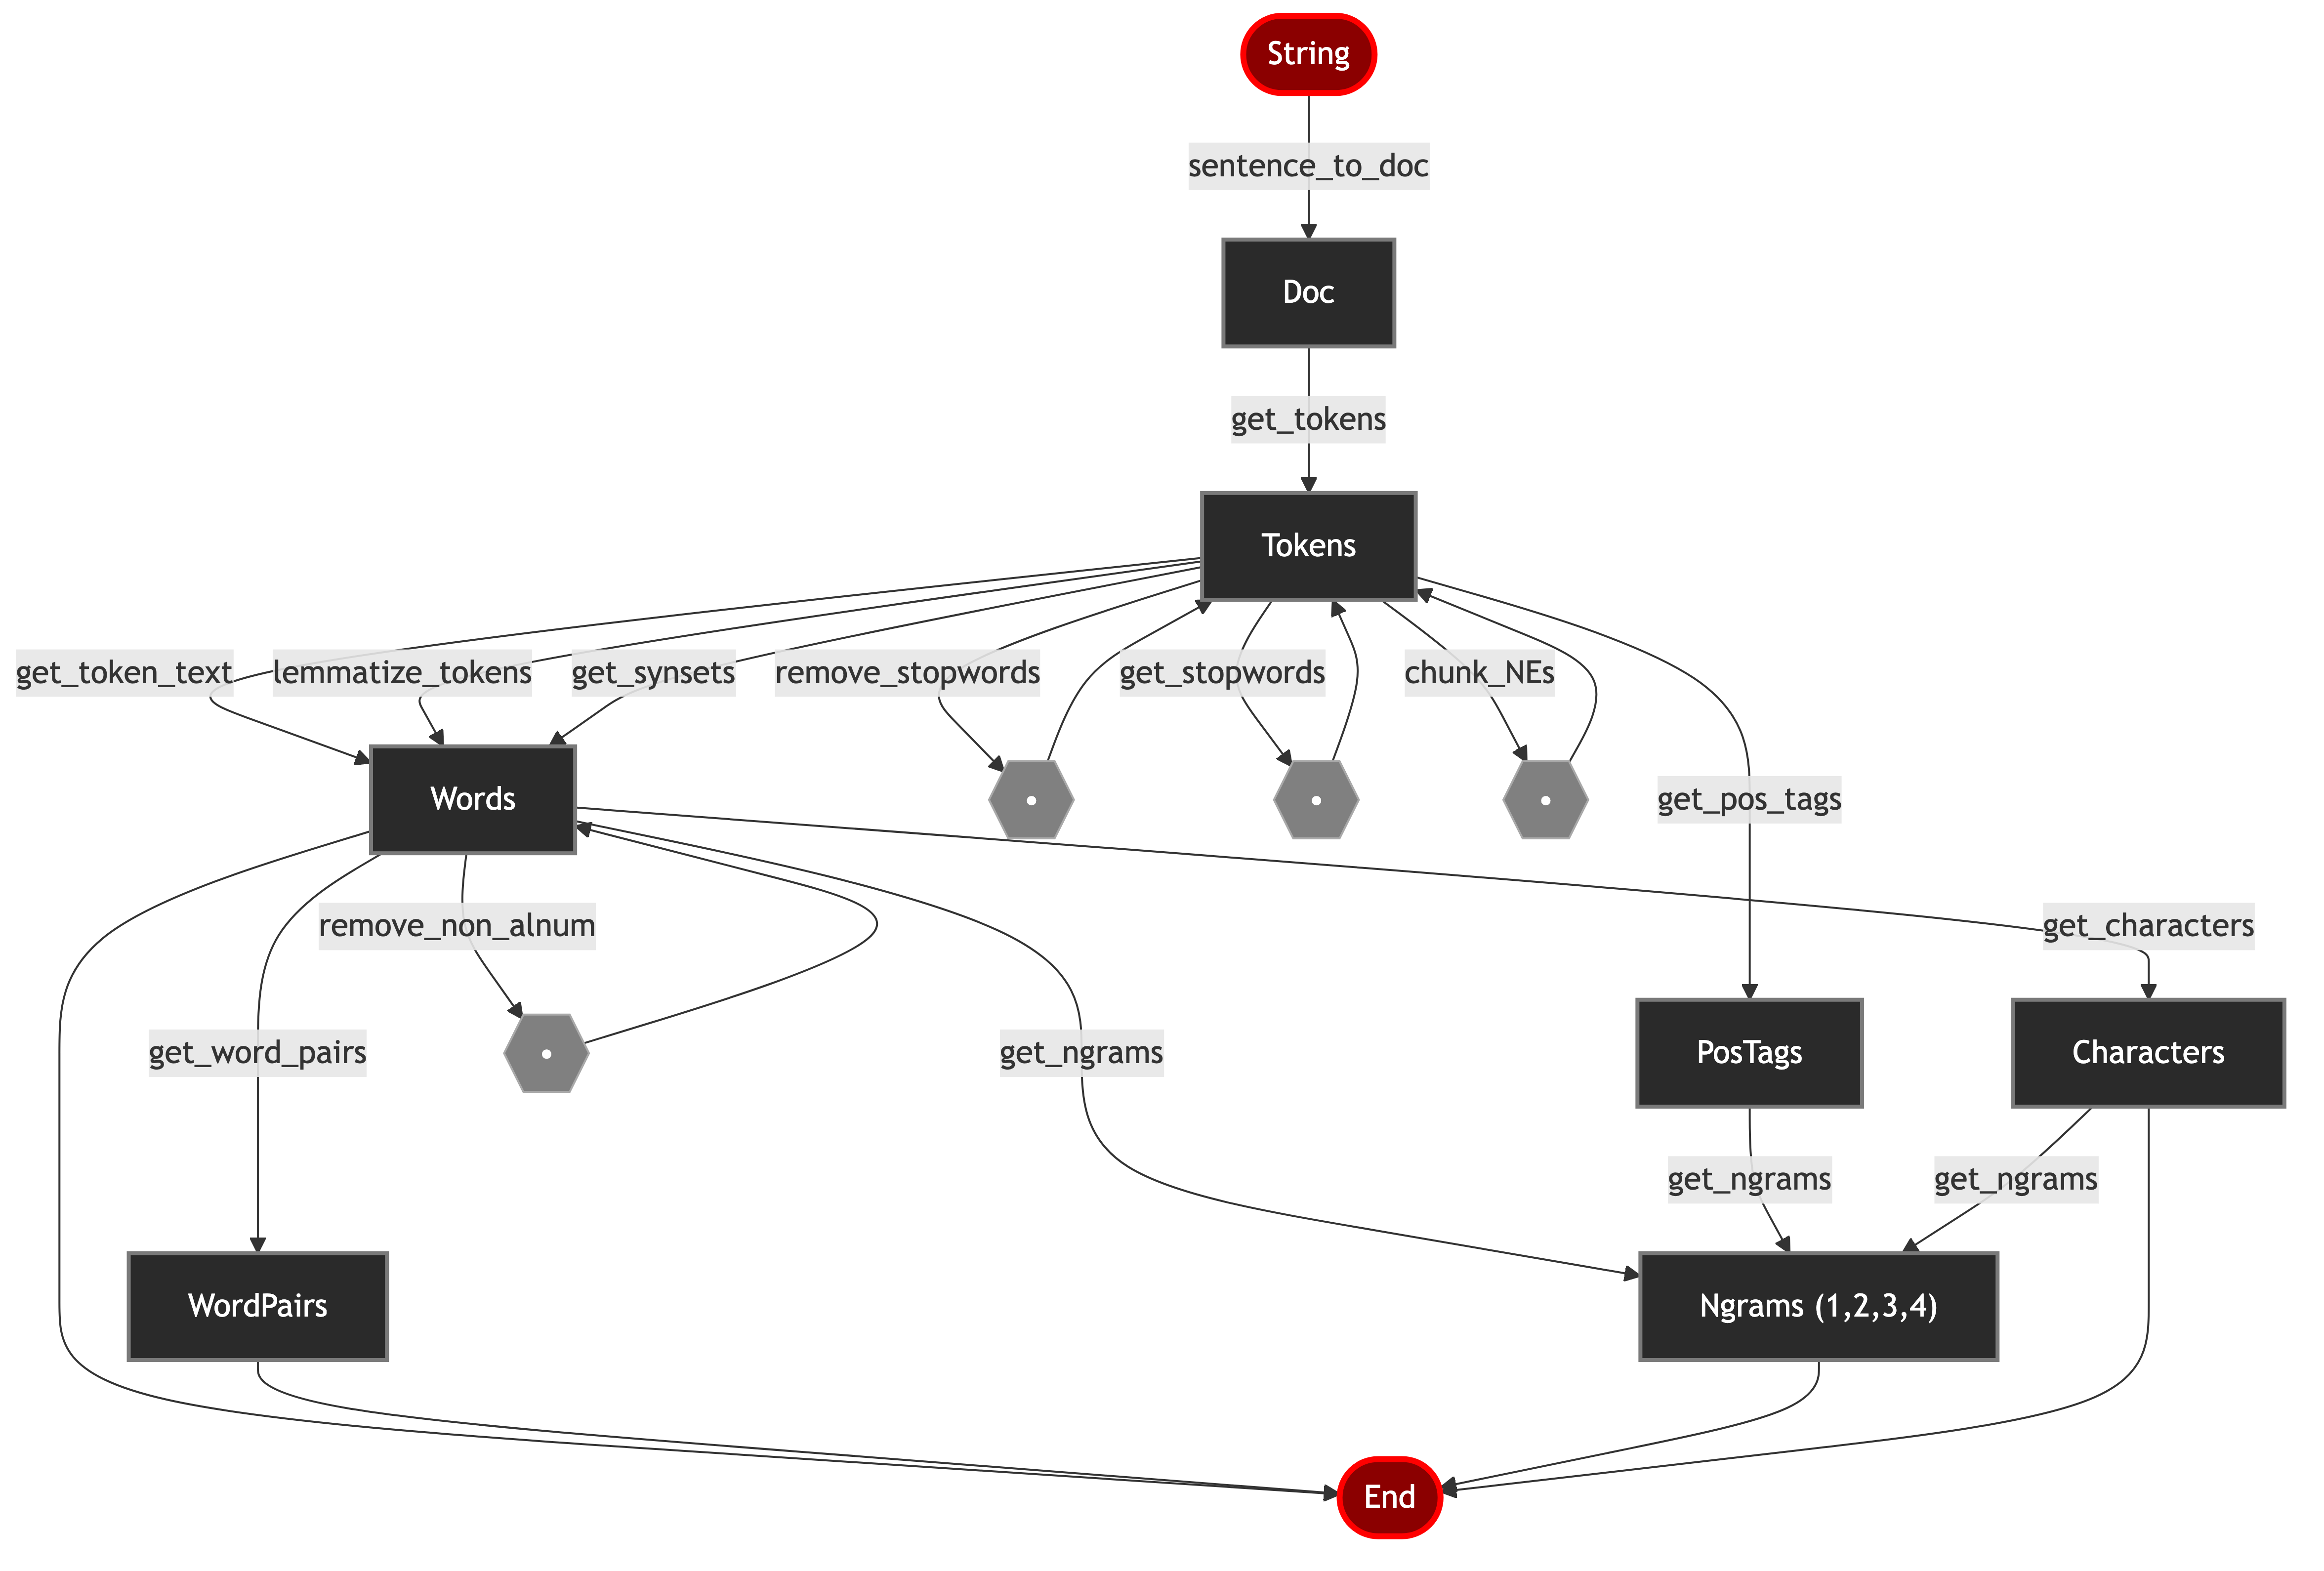
\includegraphics[width=0.9\textwidth]{figures/mermaid/permutations.md-1.png}
    \end{center}
\end{frame}

\begin{frame}[fragile]{\texttt{generate\_valid\_permutations()}}
    \begin{lstlisting}[language=Python]
# Generate all valid permutations of sentence processing steps
def generate_valid_permutations(
    functions: List[Callable] = all_functions,
) -> List[Tuple[Callable, ...]]:
    valid_permutations = []
    for n in range(1, len(functions) + 1):
        for perm in itertools.permutations(functions, n):
            if _is_valid_permutation(perm):
                valid_permutations.append(perm)
    # Add sentence_to_doc to the beginning of each permutation
    valid_permutations = (
        [tuple([sentence_to_doc]) + perm for perm in valid_permutations])
    # Add final step to each permutation (e.g. get_2grams)
    valid_permutations = (
        [new_perm for perm in valid_permutations for new_perm in add_final_step(perm)])
    return valid_permutations

    \end{lstlisting}
\end{frame}

\begin{frame}[fragile]{}
    \begin{lstlisting}[language=Python]
# Dictionary to hold function names and their input/output types
function_input_output_types: Dict[str, Tuple[Tuple[type, ...], type]] = {}

# Extract the input and output types of a function
def _extract_input_output_types(func: Callable) -> Tuple[type, type]:
    signature = inspect.signature(func)
    param_types = [param.annotation for param in signature.parameters.values()]
    return_type = signature.return_annotation
    return param_types[0], return_type

# Populate the dictionary with function names and their input/output types
for func in all_functions:
    input_types, output_type = _extract_input_output_types(func)
    function_input_output_types[func.__name__] = (input_types, output_type)


# Function to check if a permutation is valid based on input/output types
def _is_valid_permutation(perm: Tuple[Callable]) -> bool:
    if function_input_output_types[perm[0].__name__][0] != spacy.tokens.doc.Doc:
        return False
    if function_input_output_types[perm[-1].__name__][1] not in [
        Tuple[Word, ...],
        Tuple[PosTag, ...],
        Tuple[Character, ...],
    ]:
        return False
    for i in range(len(perm) - 1):
        _, current_func_output_type = function_input_output_types[perm[i].__name__]
        next_func_input_type, _ = function_input_output_types[perm[i + 1].__name__]
        if current_func_output_type != next_func_input_type:
            return False
    return True
    \end{lstlisting}
\end{frame}

\begin{frame}[fragile]{}
    \begin{lstlisting}[language=Python]
class PosTag(str): pass
class Word(str): pass
class Character(str): pass
class Ngram(Tuple[Word | Character | PosTag, ...]): pass
class WordPair(Tuple[Word, Word]): pass

def get_characters(words: Tuple[Word, ...]) -> Tuple[Character, ...]:
def get_word_pairs(words: Tuple[Word, ...]) -> Tuple[WordPair, ...]:
def sentence_to_doc(sentence: str) -> spacy.tokens.doc.Doc:
def get_tokens(doc: spacy.tokens.doc.Doc) -> Tuple[spacy.tokens.token.Token, ...]:
def get_pos_tags(tokens: Tuple[spacy.tokens.token.Token, ...]) -> Tuple[PosTag, ...]:
def lemmatize_tokens(tokens: Tuple[spacy.tokens.token.Token, ...]) -> Tuple[Word, ...]:
def get_token_text(tokens: Tuple[spacy.tokens.token.Token, ...]) -> Tuple[Word, ...]:
def get_2grams(words: Tuple[Word | Character | PosTag, ...]) -> Tuple[Ngram, ...]:
def get_3grams(words: Tuple[Word | Character | PosTag, ...]) -> Tuple[Ngram, ...]:
def get_4grams(words: Tuple[Word | Character | PosTag, ...]) -> Tuple[Ngram, ...]:
def chunk_NEs(doc: spacy.tokens.doc.Doc) -> Tuple[spacy.tokens.token.Token, ...]:
def get_synsets(tokens: Tuple[spacy.tokens.token.Token, ...]) -> Tuple[Word, ...]:
def remove_non_alnum(words: Tuple[Word, ...]) -> Tuple[Word, ...]:
def remove_stopwords(tokens: Tuple[spacy.tokens.token.Token, ...])
    -> Tuple[spacy.tokens.token.Token, ...]:
def get_stopwords(tokens: Tuple[spacy.tokens.token.Token, ...])
    -> Tuple[spacy.tokens.token.Token, ...]:
    \end{lstlisting}
\end{frame}

\begin{frame}[fragile]{Feature Extraction}
    \begin{lstlisting}[language=Python]
lexical_functions = [
    get_characters,      # Character-level patterns
    get_tokens,          # Word tokenization
    get_token_text,      # Raw word forms
    remove_non_alnum,    # Character filtering
    get_word_pairs,      # Word co-occurrences
]

semantic_functions = [
    lemmatize_tokens,    # Normalize to base meaning
    get_synsets,         # Word meanings/concepts
    chunk_NEs,           # Named entity grouping
    get_pos_tags,        # Part of speech (bridges lexical/semantic)
]

ngram_functions = [
    get_2grams,          # Bigrams
    get_3grams,          # Trigrams
    get_4grams,          # 4-grams
]

preprocessing_functions = [
    remove_stopwords,    # Filter non-content words
    get_stopwords,       # Identify non-content words
]

all_functions = lexical_functions + semantic_functions + preprocessing_functions
    \end{lstlisting}
\end{frame}

\begin{frame}[fragile]{Feature Extraction}
    Cache is king \{ \textdollar{}, \texteuro{} \}
    \begin{lstlisting}[language=Python]
@cache
def get_tokens(doc: spacy.tokens.doc.Doc) -> Tuple[spacy.tokens.token.Token, ...]:
    return tuple(token for token in doc)
    \end{lstlisting}
    \begin{itemize}
        \item Many variations in ordering result in same output
        \item This is a prime candidate for dynamic programming
        \item Caching significantly speeds up feature extraction
        \item 520 processes x 4 metrics = 2080 features
        \begin{itemize}
            \item across all \textasciitilde{}5000 sentence pairs takes \textasciitilde{}15 minutes
        \end{itemize}
    \end{itemize}
\end{frame}

\subsection{Model Training}
\begin{frame}{Model Training}
    \begin{itemize}
        \item Random Forest
        \begin{itemize}
            \item Built-in feature importance analysis
            \item Bagging allows discovery of local patterns
            \item Handles high-dimensional feature spaces well (2080 features)
            \item Resistant to overfitting
        \end{itemize}
        \item Model Configuration
        \begin{itemize}
            \item 100 trees in ensemble
            \item No max depth, since we are interested in identifying fine-grained feature importances
        \end{itemize}
    \end{itemize}
\end{frame}

\subsection{Feature Selection}
\begin{frame}{Feature Selection}
    \begin{itemize}
        \item 520 permutations x 4 metrics = 2080 features
        \item The random forest model allows us to inspect feature importances
        \item We used this to identify how important the top features are to the model
        \item We trained and validated models with different subsets of the top features
    \end{itemize}
\end{frame}

\subsection{Model Evaluation}
\begin{frame}{Model Evaluation}
    \begin{itemize}
        \item Multi-level evaluation strategy
        \begin{itemize}
            \item Initial 5-fold cross-validation on training set
            \item 80/20 train/validation split for comparing feature sets
            \item Held-out test set for final evaluation
        \end{itemize}
        \item Custom Pearson correlation scorer
        \begin{itemize}
            \item Measures linear correlation with gold standard
            \item Implemented as sklearn-compatible scoring function
            \item Allows direct comparison with published results
        \end{itemize}
    \end{itemize}
\end{frame}

% Results
\section{Results}
\begin{frame}{Results}
    \begin{itemize}
        \item \textbf{Feature Importance}
        \begin{itemize}
            \item Top 10 features account for \textasciitilde{}50\% of total importance
            \item 60\% of features (1,248) have non-zero importance
            \item Reducing to 500 features shows slight performance loss
        \end{itemize}
        \item \textbf{Feature Type Comparison}
        \begin{itemize}
            \item Combined features perform best (r = 0.735 on test)
            \item Lexical features alone achieve strong performance (r = 0.718)
            \item Semantic features show lower generalization (r = 0.640)
            \item N-grams important for generalization
        \end{itemize}
        \item \textbf{Dataset-Specific Performance}
        \begin{itemize}
            \item MSRvid highest performance (r \textgreater{} 0.80)
            \item SMTnews and SMTeuroparl lower performance (r \textless{} 0.52)
            \item Performance varies across datasets
        \end{itemize}
    \end{itemize}
\end{frame}

\begin{frame}{Top Features}
    \begin{itemize}
        \item Jaccard similarity dominates (6 of top 10)
        \item Common steps: \texttt{sentence\_to\_doc}, \texttt{lemmatize\_tokens}, \texttt{get\_characters}
        \item N-grams frequently appear, especially 2-grams
    \end{itemize}
    \begin{figure}[h]
        \centering
        \begin{tabular}{|l|l|c|}
            \hline
            \tiny{\textbf{Feature}} & \tiny{\textbf{Processing Steps}} & \tiny{\textbf{Importance}} \\
            \hline
            \tiny{score\_jaccard\_165} & \tiny{doc → tokens → stopwords → lemma → chars → 2gram} & \tiny{0.197} \\
            \tiny{score\_cosine\_257} & \tiny{doc → NEs → stopwords → lemma → chars → 2gram} & \tiny{0.089} \\
            \tiny{score\_cosine\_165} & \tiny{doc → tokens → stopwords → lemma → chars → 2gram} & \tiny{0.069} \\
            \tiny{score\_jaccard\_258} & \tiny{doc → NEs → stopwords → lemma → chars → 3gram} & \tiny{0.033} \\
            \tiny{score\_cosine\_258} & \tiny{doc → NEs → stopwords → lemma → chars → 3gram} & \tiny{0.022} \\
            \tiny{score\_jaccard\_256} & \tiny{doc → NEs → stopwords → lemma → chars} & \tiny{0.021} \\
            \tiny{score\_jaccard\_257} & \tiny{doc → NEs → stopwords → lemma → chars → 2gram} & \tiny{0.021} \\
            \tiny{score\_cosine\_166} & \tiny{doc → tokens → stopwords → lemma → chars → 3gram} & \tiny{0.021} \\
            \tiny{score\_jaccard\_97} & \tiny{doc → NEs → lemma → chars → 2gram} & \tiny{0.019} \\
            \tiny{score\_jaccard\_41} & \tiny{doc → tokens → lemma → chars → 2gram} & \tiny{0.019} \\
            \hline
        \end{tabular}
    \end{figure}
\end{frame}

\begin{frame}{Dataset-Specific Performance}
    \begin{center}
        \begin{tabular}{|l|c|c|c|c|}
            \hline
            \textbf{Dataset} & \textbf{Without} & \textbf{Without} & \textbf{Without} & \textbf{All} \\
            & \textbf{Semantic} & \textbf{Lexical} & \textbf{N-grams} & \textbf{Features} \\
            \hline
            MSRpar & 0.646 & 0.533 & 0.577 & 0.643 \\
            MSRvid & 0.813 & 0.811 & 0.807 & 0.839 \\
            Teuroparl & 0.521 & 0.437 & 0.475 & 0.495 \\
            OnWN & 0.671 & 0.470 & 0.623 & 0.647 \\
            SMTnews & 0.451 & 0.367 & 0.438 & 0.420 \\
            \hline
            All & 0.718 & 0.639 & 0.686 & 0.734 \\
            \hline
        \end{tabular}
    \end{center}
    \begin{itemize}
        \item Key Observations:
        \begin{itemize}
            \item MSRvid shows consistently high performance (r \textgreater{} 0.80)
            \item SMTnews and Teuroparl show lower performance (r \textless{} 0.52)
            \item Performance varies significantly by dataset
            \item Lexical features most important across all datasets
        \end{itemize}
    \end{itemize}
\end{frame}

% Conclusions
\section{Conclusions}
\begin{frame}{Conclusions}
    \begin{itemize}
        \item TODO
    \end{itemize}
\end{frame}

\end{document}
